\section{Additional internal-routing diagnostics}
\label{app:internal_routing}

\paragraph{Evaluation and statistics.}
We inspect the fixed circular-cylinder Hopf and Periodic specialists on their
held-out autonomous rollout windows. The Periodic analysis uses 13 fixed windows
at each of four held-out Reynolds numbers ($52$ windows, $K=48$); the Hopf
analysis uses five fixed windows at each of three held-out Reynolds numbers
($15$ windows, $K=56$). Each statistic uses one routing record per macro-step,
taken at its first integration stage, giving $2496$ Periodic and $840$ Hopf
decisions per channel. These are macro-step statistics, not a count of all
right-hand-side evaluations. Overlapping windows are not treated as independent
trajectories, and no diagnostic is used for model selection.

For $N$ decisions, let $I_{n,e}$ indicate whether routed expert $e$ is selected,
with group identity included in $e$. We report normalized activation frequency
$f_e=\sum_n I_{n,e}/(2N)$ and mean routing mass
$m_e=N^{-1}\sum_n\omega_{n,e}I_{n,e}$, retaining zero-use experts.
The utilization entropy is
$H=-\sum_{e:f_e>0}f_e\log f_e/\log N_E$, where $N_E$ counts all routed
experts in the corresponding channel. Distinct pairs include group identity
but ignore the order of the two selected experts. The shared/routed mixture
coefficient is fixed by architecture; a shared expert is always active in the
selected group, while the routed component is allocated conditionally.
For both specialists here, the shared coefficient is $4/7$ and
$\sum_e m_e=3/7$.
Routing mass is a mixing coefficient, not the norm of an expert's output or
its causal contribution to prediction.
Figure identifiers such as \texttt{g0:e0} enumerate routed experts only;
they are distinct from the shared-expert index $0$ in
Eq.~(\plaineqref{eq:app_channel_sparse_moe}).

\begin{table}[htbp]
\centering
\caption{Post-hoc internal-routing statistics on held-out autonomous rollout
windows. Entropy is a descriptive utilization statistic, not a performance
score. A fixed Top-2 pair has nonzero entropy; the two specialists also have
different numbers of available groups.}
\label{tab:internal_routing_summary}
\small
\setlength{\tabcolsep}{5pt}
\begin{tabular}{@{}llrrrr@{}}
\toprule
Specialist & Channel & Used experts & Distinct pairs & Dominant pair (\%) & $H$ \\
\midrule
Hopf & Velocity & 2/6 & 1 & 100.00 & 0.387 \\
     & Pressure & 2/6 & 1 & 100.00 & 0.387 \\
\addlinespace
Periodic & Velocity & 18/18 & 33 & 16.27 & 0.929 \\
         & Pressure & 14/18 & 16 & 31.25 & 0.784 \\
\bottomrule
\end{tabular}
\end{table}

\paragraph{Hopf routing profile.}
The Hopf specialist exhibits a different sparse-routing pattern from the
Periodic model. It contains one group by construction and selects a fixed
channel-specific pair over the evaluated windows: $(e_1,e_3)$ for velocity
and $(e_2,e_4)$ for pressure. The same selected pairs occur at all four
integration stages. Velocity expert $e_3$ accounts for approximately
$99.93\%$ of pooled routed mass; pressure expert $e_2$ accounts for
$84.16\%$. The pressure pair nevertheless retains variable internal
weighting: the mean mass assigned to the secondary pressure expert $e_4$
increases markedly across the three held-out Reynolds numbers.
Thus, routing profiles are chart dependent: Periodic uses a broad set of
configurations, whereas Hopf uses stable sparse support with nonuniform
mixing weights. The sole Hopf group is a structural choice, not evidence of
competition collapsing among multiple groups.

\paragraph{Periodic rollout-position diagnostic.}
Figure~\ref{fig:periodic_routing_step} reports routed-expert mass as a function
of normalized rollout position, pooling the same 52 fixed held-out windows.
This is a temporal routing diagnostic, not an estimate of physical oscillation
phase. Together with Figure~\ref{fig:periodic_internal_routing}, it describes
conditional allocation within the Periodic specialist without assigning
physical semantics to expert identities.

\begin{figure}[htbp]
\centering
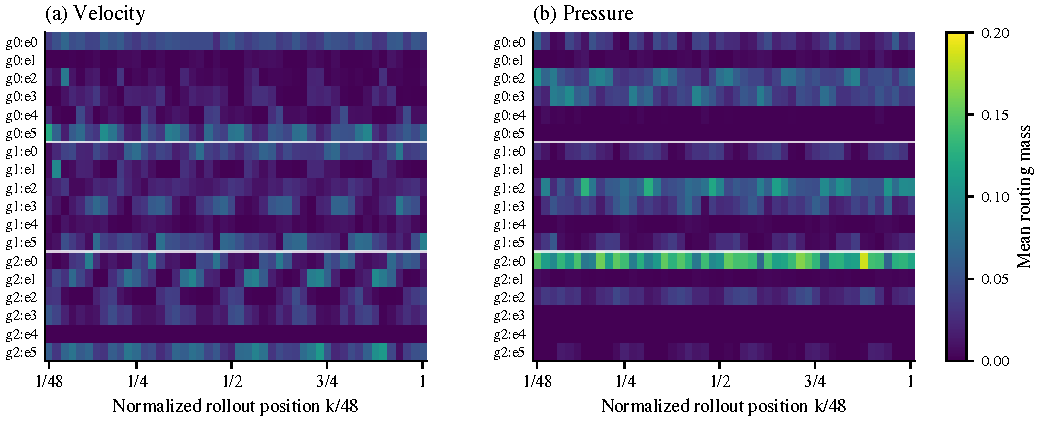
\includegraphics[width=\linewidth]{figures/periodic_rollout_step_routing.pdf}
\caption{Routing mass across autonomous rollout position for the
circular-cylinder Periodic specialist. Each column averages the corresponding
macro-step decision over the fixed held-out windows; all routed-expert rows
are retained. The horizontal coordinate denotes normalized rollout position
$k/48$ and is not interpreted as physical oscillation phase.}
\label{fig:periodic_routing_step}
\end{figure}
